%
% File acl2015.tex
%
% Contact: car@ir.hit.edu.cn, gdzhou@suda.edu.cn
%%
%% Based on the style files for ACL-2014, which were, in turn,
%% Based on the style files for ACL-2013, which were, in turn,
%% Based on the style files for ACL-2012, which were, in turn,
%% based on the style files for ACL-2011, which were, in turn, 
%% based on the style files for ACL-2010, which were, in turn, 
%% based on the style files for ACL-IJCNLP-2009, which were, in turn,
%% based on the style files for EACL-2009 and IJCNLP-2008...

%% Based on the style files for EACL 2006 by 
%%e.agirre@ehu.es or Sergi.Balari@uab.es
%% and that of ACL 08 by Joakim Nivre and Noah Smith

\documentclass[11pt]{article}
\usepackage{acl2015}
\usepackage{times}
\usepackage{url}
\usepackage{latexsym}
\usepackage[utf8]{inputenc}
\usepackage{graphicx}
\usepackage{color}
\usepackage[colorinlistoftodos,prependcaption,textsize=tiny]{todonotes}
\usepackage[round]{natbib}
\usepackage[tight,footnotesize]{subfigure}
\usepackage[caption=false,font=small,margin=0.5cm]{caption}
\usepackage{tabularx}
\usepackage{array}
\usepackage{titlesec}
\usepackage{blindtext}
\usepackage{threeparttable}

\title{Title here}

\author{Author 1 \qquad Author 2\thanks{\hspace{0.2cm} AUthor 2 is also with ...} \\ Affiliation line 1 \\ Afilliation line 2 \\ Location \\ {\tt \{author1,author2\}@domain.edu} \\}

% TODO
\newcommand{\unsure}[2][1=]{\todo[linecolor=red,backgroundcolor=red!25,bordercolor=red,#1]{#2}}
\newcommand{\change}[2][1=]{\todo[linecolor=blue,backgroundcolor=blue!25,bordercolor=blue,#1]{#2}}
\newcommand{\info}[2][1=]{\todo[linecolor=OliveGreen,backgroundcolor=OliveGreen!25,bordercolor=OliveGreen,#1]{#2}}
\newcommand{\improvement}[2][1=]{\todo[linecolor=Plum,backgroundcolor=Plum!25,bordercolor=Plum,#1]{#2}}
\newcommand{\thiswillnotshow}[2][1=]{\todo[disable,#1]{#2}}

\newcommand{\cit}[0]{\todo[linecolor=blue,backgroundcolor=blue!25,bordercolor=blue]{CITATION NEEDED}}

\begin{document}

% COLUMN TYPES FOR TABULARX
\newcolumntype{L}[1]{>{\raggedright\let\newline\\\arraybackslash\hspace{0pt}}p{#1}}
\newcolumntype{C}[1]{>{\centering\let\newline\\\arraybackslash\hspace{0pt}}p{#1}}
\newcolumntype{R}[1]{>{\raggedleft\let\newline\\\arraybackslash\hspace{0pt}}p{#1}}

\maketitle

\begin{abstract}
%\boldmath
\blindtext
\end{abstract}

\section{Introduction}

\blindtext

\section{Section 1}

Example of citation: \cite{bengio_et_al_2003}.

\blindtext

\renewcommand{\arraystretch}{1.3}
\begin{table*}[h]
\small
\begin{tabularx}{\textwidth}{|L{15mm}|X|L{15mm}|X|}
\hline
\textbf{Col 1 (fixed-width)} & \textbf{Col 2 (variable width)} & \textbf{Col 3 (fixed width)}  & \textbf{Col 4 (variable width)} \\ \hline 
foo bar & foo-bar baz & foo bar baz quux & foo bar baz. \\ \hline
\end{tabularx}
\caption{Table caption here.}
\end{table*}

\begin{figure}[!htb]
\begin{center}
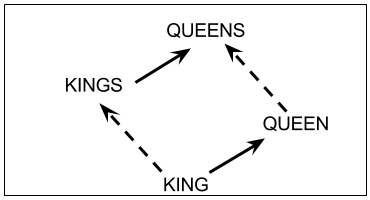
\includegraphics[width=6cm]{pictures/word2vec2.png}
\caption{Image caption here}
\vspace{-1.5em}
\label{fig1}
\end{center}
\end{figure}

\section{Conclusion}

\blindtext

\section{Further Work}

\blindtext

% include your own bib file like this:
\bibliographystyle{plainnatsimple}
\bibliography{ref}

\printbibliography


\end{document}